\section*{Questão 4: Voltando à origem}
Considere uma cadeia de Markov cujo espaço de estados é um láttice de duas dimensões sobre os números naturais, ou seja, $S = \{(i, j) \mid i \geq 1, j \geq 1\}$. Cada estado pode transicionar para um de seus vizinhos no láttice. Entretanto, se afastar da origem (se movimentar para o norte ou para o leste) tem probabilidade $p/2$, e se aproximar da origem tem probabilidade $(1-p)/2$, onde $p$ é um parâmetro do modelo (nas bordas, utilize self-loops). Assuma que $p \in \{0.25, 0.35, 0.45\}$.

\begin{enumerate}
    \item Construa um simulador para essa cadeia de Markov.
    \begin{resposta}
        A representação da Cadeia de Markov pode ser vista na figura abaixo:
        \begin{center}\begin{tikzpicture}[->, >=stealth, node distance=2cm,
                every state/.style={circle, draw, minimum size=1.2cm},
                shorten >=1pt]

            % Linha 1 (j = 1)
            \node[state] (11) at (0, 0) {(1,1)};
            \node[state] (12) at (3, 0) {(1,2)};
            \node[state] (13) at (6, 0) {(1,3)};
            \node at (9, 0) (dots1) {\(\cdots\)};
            
            % Linha 2 (j = 2)
            \node[state] (21) at (0, 3) {(2,1)};
            \node[state] (22) at (3, 3) {(2,2)};
            \node[state] (23) at (6, 3) {(2,3)};
            \node at (9, 3) (dots2) {\(\cdots\)};
            
            % Linha 3 (j = 3)
            \node[state] (31) at (0, 6) {(3,1)};
            \node[state] (32) at (3, 6) {(3,2)};
            \node[state] (33) at (6, 6) {(3,3)};
            \node at (9, 6) (dots3) {\(\cdots\)};
            
            % Pontos verticais indicando crescimento para cima
            \node at (0,9) (vdots1) {\(\vdots\)};
            \node at (3,9) (vdots2) {\(\vdots\)};
            \node at (6,9) (vdots3) {\(\vdots\)};
            
            % Transições norte
            \draw[bend left=15] (11) to node[left] {\(\frac{p}{2}\)} (21);
            \draw[bend left=15] (12) to node[left] {\(\frac{p}{2}\)} (22);
            \draw[bend left=15] (13) to node[left] {\(\frac{p}{2}\)} (23);

            \draw[bend left=15] (21) to node[left] {\(\frac{p}{2}\)} (31);
            \draw[bend left=15] (22) to node[left] {\(\frac{p}{2}\)} (32);
            \draw[bend left=15] (23) to node[left] {\(\frac{p}{2}\)} (33);

            \draw[bend left=15] (31) to node[left] {\(\frac{p}{2}\)} (vdots1);
            \draw[bend left=15] (32) to node[left] {\(\frac{p}{2}\)} (vdots2);
            \draw[bend left=15] (33) to node[left] {\(\frac{p}{2}\)} (vdots3);
            
            % Transições sul
            \draw[bend left=15] (21) to node[right] {\(\frac{1-p}{2}\)} (11);
            \draw[bend left=15] (22) to node[right] {\(\frac{1-p}{2}\)} (12);
            \draw[bend left=15] (23) to node[right] {\(\frac{1-p}{2}\)} (13);

            \draw[bend left=15] (31) to node[right] {\(\frac{1-p}{2}\)} (21);
            \draw[bend left=15] (32) to node[right] {\(\frac{1-p}{2}\)} (22);
            \draw[bend left=15] (33) to node[right] {\(\frac{1-p}{2}\)} (23);

            \draw[bend left=15] (vdots1) to node[right] {\(\frac{1-p}{2}\)} (31);
            \draw[bend left=15] (vdots2) to node[right] {\(\frac{1-p}{2}\)} (32);
            \draw[bend left=15] (vdots3) to node[right] {\(\frac{1-p}{2}\)} (33);
            
            % Transições leste
            \draw[bend left=15] (11) to node[above] {\(\frac{p}{2}\)} (12);
            \draw[bend left=15] (12) to node[above] {\(\frac{p}{2}\)} (13);
            \draw[bend left=15] (13) to node[above] {\(\frac{p}{2}\)} (dots1);

            \draw[bend left=15] (21) to node[above] {\(\frac{p}{2}\)} (22);
            \draw[bend left=15] (22) to node[above] {\(\frac{p}{2}\)} (23);
            \draw[bend left=15] (23) to node[above] {\(\frac{p}{2}\)} (dots2);

            \draw[bend left=15] (31) to node[above] {\(\frac{p}{2}\)} (32);
            \draw[bend left=15] (32) to node[above] {\(\frac{p}{2}\)} (33);
            \draw[bend left=15] (33) to node[above] {\(\frac{p}{2}\)} (dots3);
            
            % Transições oeste
            \draw[bend left=15] (12) to node[below] {\(\frac{1-p}{2}\)} (11);
            \draw[bend left=15] (13) to node[below] {\(\frac{1-p}{2}\)} (12);
            \draw[bend left=15] (dots1) to node[below] {\(\frac{1-p}{2}\)} (13);

            \draw[bend left=15] (22) to node[below] {\(\frac{1-p}{2}\)} (21);
            \draw[bend left=15] (23) to node[below] {\(\frac{1-p}{2}\)} (22);
            \draw[bend left=15] (dots2) to node[below] {\(\frac{1-p}{2}\)} (23);

            \draw[bend left=15] (32) to node[below] {\(\frac{1-p}{2}\)} (31);
            \draw[bend left=15] (33) to node[below] {\(\frac{1-p}{2}\)} (32);
            \draw[bend left=15] (dots3) to node[below] {\(\frac{1-p}{2}\)} (33);

            % Self-loops nas bordas
            \draw (11) edge[loop left] node[left] {\(\frac{1-p}{2}\)} (11);
            \draw (21) edge[loop left] node[left] {\(\frac{1-p}{2}\)} (21);
            \draw (31) edge[loop left] node[left] {\(\frac{1-p}{2}\)} (31);

            \draw (11) edge[loop below] node[below] {\(\frac{1-p}{2}\)} (11);
            \draw (12) edge[loop below] node[below] {\(\frac{1-p}{2}\)} (12);
            \draw (13) edge[loop below] node[below] {\(\frac{1-p}{2}\)} (13);

        \end{tikzpicture}\end{center}
    
    Os elementos da Matriz de Transição $P$ podem ser calculados da seguinte forma:
    $$
    P_{(i,j),(i',j')} = \begin{cases}
    \frac{p}{2} & \text{se } i' = i+1 \land j' = j \quad \text{(norte)} \\
    \frac{p}{2} & \text{se } i' = i \land j' = j+1 \quad \text{(leste)} \\
    \frac{1-p}{2} & \text{se } i > 1 \land i' = i-1 \land j' = j \quad \text{(sul)} \\
    \frac{1-p}{2} & \text{se } j > 1 \land i' = i \land j' = j-1 \quad \text{(oeste)} \\
    \frac{1-p}{2} & \text{se } i = 1 \land i' = i \land j' = j \quad \text{(borda inferior)} \\
    \frac{1-p}{2} & \text{se } j = 1 \land i' = i \land j' = j \quad \text{(borda esquerda)} \\
    0 & \text{caso contrário}
    \end{cases}
    $$

    Como a cadeia de Markov possui um número infinito de estados, a matriz de transição completa não pode ser armazenada integralmente na memória do computador. No entanto, para cada estado, conhecemos seus vizinhos e as respectivas probabilidades de transição. Assim, é possível implementar um código que, com base no estado atual, gera o próximo estado como um ``dado enviesado'', ou seja, uma amostra aleatória com probabilidades associadas a cada vizinho.

    Ou seja, a cada iteração, o simulador deverá, com base no estado atual $(i, j)$, escolher um dos vizinhos $(i', j')$ com probabilidade $P_{(i,j),(i',j')}$. Para isso, o código pode gerar um número aleatório entre 0 e 1 e compará-lo com a distribuição acumulada das probabilidades dos vizinhos. O próximo estado será aquele cuja faixa acumulada contém o número gerado, simulando assim um dado enviesado de acordo com as probabilidades de transição.

    \begin{center}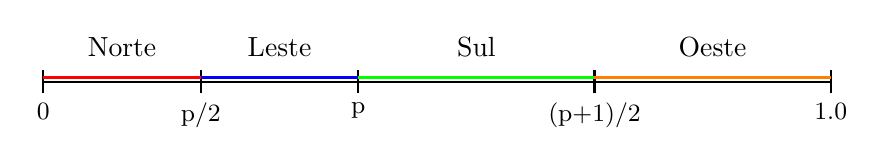
\begin{tikzpicture}
        \draw[thick] (0,0) -- (10,0);  % base line

        % vertical ticks and labels
        \foreach \x/\label in {0/{0}, 2/{p/2}, 4/{p}, 7/{(p+1)/2}, 10/{1.0}} {
            \draw[thick] (\x, -0.15) -- (\x, 0.15);
            \node[below] at (\x, -0.15) {\small \label};
        }

        % segments and labels
        \node[above] at (1, 0.2) {Norte};
        \node[above] at (3, 0.2) {Leste};
        \node[above] at (5.5, 0.2) {Sul};
        \node[above] at (8.5, 0.2) {Oeste};

        \draw[very thick, red] (0,0.05) -- (2,0.05);
        \draw[very thick, blue] (2,0.05) -- (4,0.05);
        \draw[very thick, green] (4,0.05) -- (7,0.05);
        \draw[very thick, orange] (7,0.05) -- (10,0.05);
    \end{tikzpicture}\end{center}

    \end{resposta}

    \item Utilize o simulador para estimar a distribuição estacionária da origem (estado $(1,1)$), ou seja $\pi_{1,1}$, para cada valor de $p$. Dica: utilize os tempos de retorno!
    \begin{resposta}
        Pelo Teorema Ergódico forte, se a Cadeia de Markov é irredutível, aperiódica e com distribuição estacionária $\pi$, temos:
        $$\lim_{k \to \infty} \frac{1}{k} \sum_{t=0}^{k-1} f(X_t) = E_\pi [f(X_t)],$$
        onde $f(X_t)$ é uma função qualquer de $X_t$ e $E_\pi [f(X_t)]$ é o valor esperado de $f(X_t)$ sob a distribuição estacionária $\pi$.

        Fazendo $f(X_t) = I(X_t)$, uma função indicadora que retorna $1$ se $X_t = (1,1)$ e $f(X_t) = 0$ caso contrário, temos que:
        
        $$\lim_{k \to \infty} \frac{1}{k} \sum_{t=0}^{k-1} I(X_t) = E_\pi [I(X_t)] = \pi_{1,1}\times1 + (1-\pi_{1,1})\times0 = \pi_{1,1}$$

        Com isso, podemos estimar a distribuição estacionária $\pi_{1,1}$ apenas simulando a cadeia de Markov por um número de passos suficientemente grande, contando quantas vezes o estado $(1,1)$ foi visitado e dividindo pelo número total de passos do caminho amostral. Assim, para $10^7$ passos, temos:
        \begin{itemize}
            \item Para $p = 0{,}25$, a estimativa de $\pi_{(1,1)}$ foi:
            $ \boxed{\pi_{(1,1)} \approx 0{,}4447} $
            
            \item Para $p = 0{,}35$, a estimativa de $\pi_{(1,1)}$ foi:
            $ \boxed{\pi_{(1,1)} \approx 0{,}2137} $

            \item Para $p = 0{,}45$, a estimativa de $\pi_{(1,1)}$ foi:
            $ \boxed{\pi_{(1,1)} \approx 0{,}0328} $
        \end{itemize}

    \end{resposta}
    \item Seja $d(t)$ o valor esperado da distância (de Manhattan) entre $X_t$ (o estado no tempo $t$) e a origem. Utilize o simulador para estimar $d(t)$ para $t \in \{10, 100, 1000\}$, para cada valor de $p$. O que você pode concluir?
    \begin{resposta}
        A distância de Manhattan entre $X_t=(i_t, j_t)$ e a origem $(1,1)$ é dada por:
        $$d_t = |i_t - 1| + |j_t - 1|$$

        As  estimativas de $d(t)$ para $t \in \{10, 100, 1000\}$, para cada valor de $p$ podem ser obtidas simulando, para cada valor de $p$, a cadeia de Markov por $1000$ passos e calculando a distância de Manhattan entre o estado atual e a origem. Como $d(t)$ é uma variável aleatória, podemos obter uma estimativa mais precisa rodando a simulação 30 vezes para cada valor de $p$ e calculando a média das distâncias obtidas. Assim, temos:

        \begin{center}
            \begin{tabular}{|c|c|c|c|}
            \hline
            $p$ & $d(10)$ & $d(100)$ & $d(1000)$ \\
            \hline
            0.25 & 2.70 & 3.10 & 3.00 \\
            0.35 & 3.53 & 4.57 & 4.00 \\
            0.45 & 4.50 & 8.97 & 11.40 \\
            \hline
        \end{tabular}

        \small
        OBS: os valores são decimais por ser uma média de 30 simulações.
\end{center}

    Podemos concluir que, quanto maior o valor de $p$, mais os estados tendem a se afastar da origem ao longo do tempo. Isso ocorre porque a probabilidade de se mover para o norte ou para o leste aumenta com $p$, favorecendo direções que se afastam da origem, enquanto a probabilidade de se mover para o sul ou para o oeste, que aproximam o processo da origem, diminui.

    \end{resposta}
\end{enumerate}